\documentclass[10pt,a4paper]{article}
\usepackage[utf8]{inputenc}
\usepackage{amsmath}
\usepackage{amsfonts}
\usepackage{amssymb}
\usepackage{palatino}
\usepackage[left=2.5cm,right=2.5cm,top=2.5cm,bottom=2.5cm]{geometry}
\usepackage{geometry}
\usepackage{listings}
\usepackage{amsmath,amsthm}
\usepackage{extpfeil}
\usepackage{indentfirst}
\usepackage{mathptmx}
\usepackage{subfig}
\usepackage{graphicx}
\usepackage{hyperref}
\usepackage{diagbox}
\usepackage{cite}
\global\long\def\d{\text{d}}
\newtheorem{proposition}{Proposition}
\newtheorem{definition}{Definition}
\newtheorem{corollary}{Corollary}
\newtheorem{claim}{Claim}
\newtheorem{theorem}{Theorem}
\newtheorem{lemma}{Lemma}
\newtheorem{fact}{Fact}
%\usepackage{booktabs}
%\usepackage{lipsum}
\title{DSGA-1011 Natural Language Processing with Representation Learning Homework 1
}
\author{Xintian Han (xh1007)}
\begin{document}
\maketitle
\section{Bag of N-Gram Document Classification} 
We build a bag of n-grams model for predicting the sentiment of the movie reviewers given the textual review for the movie. We use IMDB review dataset consisting of 25,000 train and 25,000 test movie reviews scraped from IMDB website. We split the train dataset into 20,000 train examples and 5,000 validation examples. We perform the hyperparameter tuning on the validation set and report the result of the best model on the test set. We use the following set of hyperparameters.
\begin{itemize}
\item Tokenization schemes of the dataset: 
\begin{itemize}
\item 'en\_core\_web\_sm'	
\end{itemize}
\item Model hyperparameters:
\begin{itemize}
\item Vary n for n-gram (n=1, 2, 3, 4)
\item vocabulary size (5000, 10000, 20000)
\item embedding size (100, 200, 500)
\end{itemize}
\item Optimization hyperparameters:
\begin{itemize}
\item Optimizer itself (SGD vs Adam)
\item Learning rate [0.1, 0.01, 0.001]
\item Whether or not you use linear annealing of learning rate (learning rate is reduced linearly over the course of training).	
\end{itemize}
\end{itemize}
For n-grams, there are two strategies. One is using only n-gram; the other is using all the k-gram until n, i.e. 4-grams including 1,2,3,4-grams. We consider both two strategies. So there are 7 choices of n-grams. We denote all\_ngram to be indicator of using all of the n-grams. There are total $7\times 3 \times 3\times 2 \times 3 \times 2 = 756$ different combinations. We first perform the ablation study. We also did an enumerative study but it took too long time and did not finish in two days. We keep the partial results of learning curves and training output in the folder and the notebook $\texttt{enumerative\_search.iynb}$. Unfortunately, we could not finish the enumerative search. The main work in this report is based on ablation study in $\texttt{hw1.ipynb}$. The github link is \href{https://github.com/XintianHan/nlp_2018}{https://github.com/XintianHan/nlp\_2018}.
\subsection{Vary Vocabulary Size and Embedding Size,  and Fix the Others}
We use n-gram = unigram, Adam, fixed-learning rate = 0.001, test vocabulary size and embedding size.
The accuracy on the validation set is shown in Table \ref{tab: vocab_emb}. 
\begin{table}[!ht]
\centering
\begin{tabular}{|l|c|c|c|}
\hline
Accuracy& 	vocab\_size = 5000 & vocab\_size = 10000 &vocab\_size = 20000 \\ \hline
emd\_size = 100& 83.2 & 83.04 & 82.94\\ \hline
emd\_size = 200 & 83.56 & 82.78 & 82.48\\ \hline
emd\_size = 500 & 82.8 & 81.54 & 81.54 \\ \hline
\end{tabular}
\caption{\label{tab: vocab_emb} Accuracy on Validation Set When We Vary Vocabulary Size and Embedding Size,  and Fix the Others.}
\end{table}
\begin{figure}[!ht]
\centering
\subfloat[(5000,100)]{
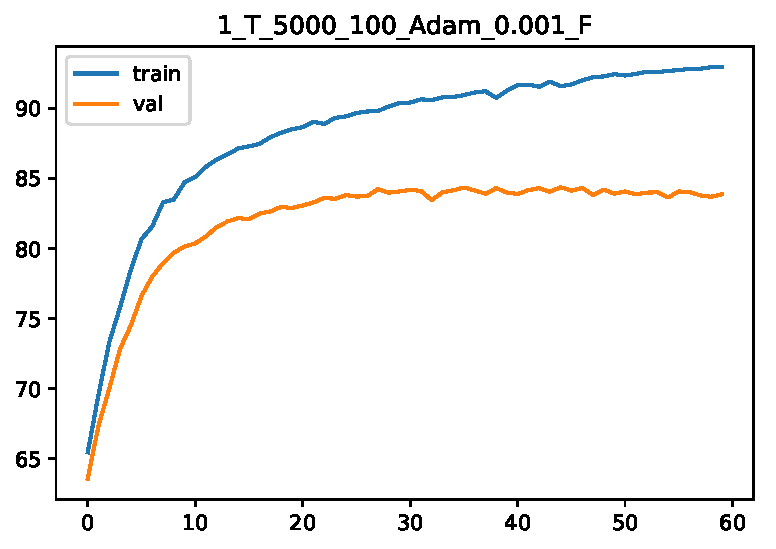
\includegraphics[width = 3cm]{1_T_5000_100_Adam_0001_F.pdf}
}
\subfloat[(10000,100)]{
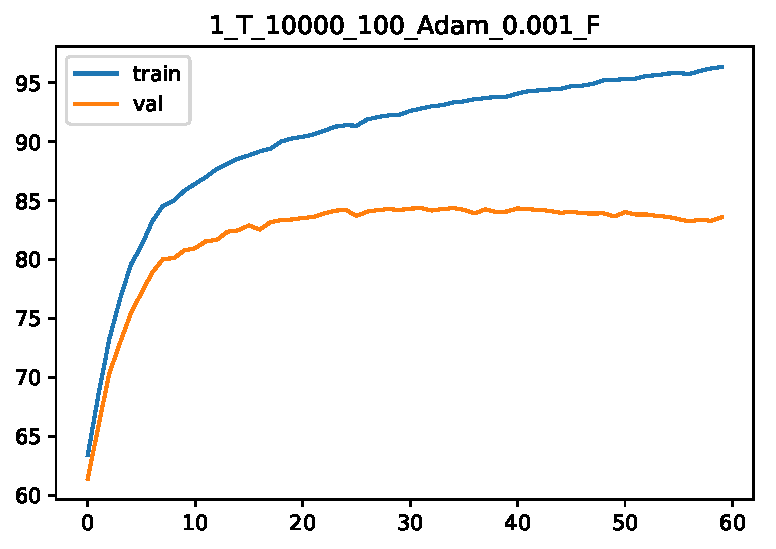
\includegraphics[width = 3cm]{1_T_10000_100_Adam_0001_F.pdf}
}	
\subfloat[(20000,100)]{
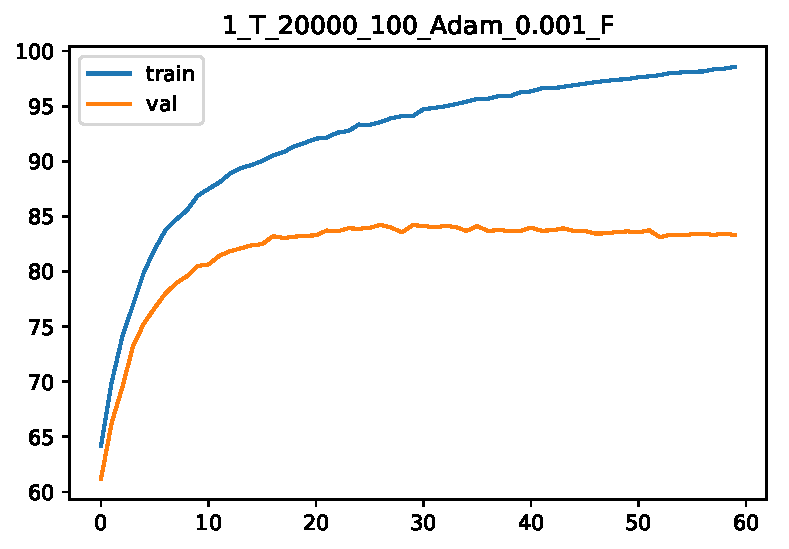
\includegraphics[width = 3cm]{1_T_20000_100_Adam_0001_F.pdf}
}
\subfloat[(5000,200)]{
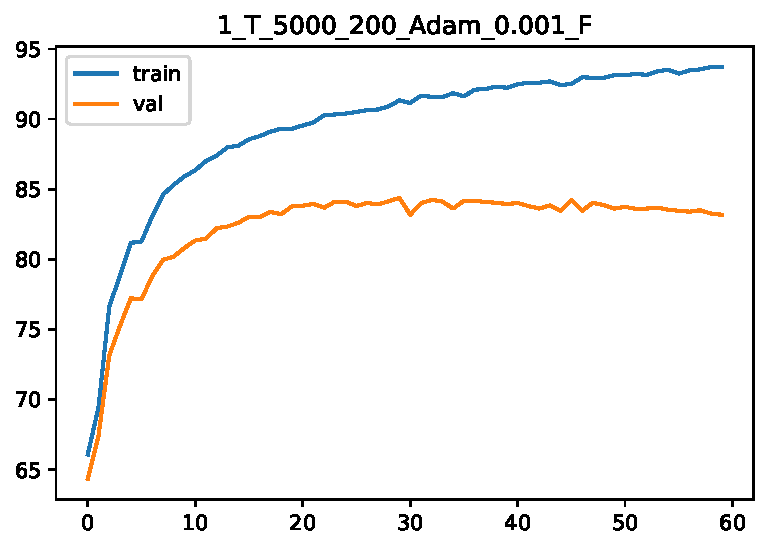
\includegraphics[width = 3cm]{1_T_5000_200_Adam_0001_F.pdf}
}		
\subfloat[(10000,200)]{
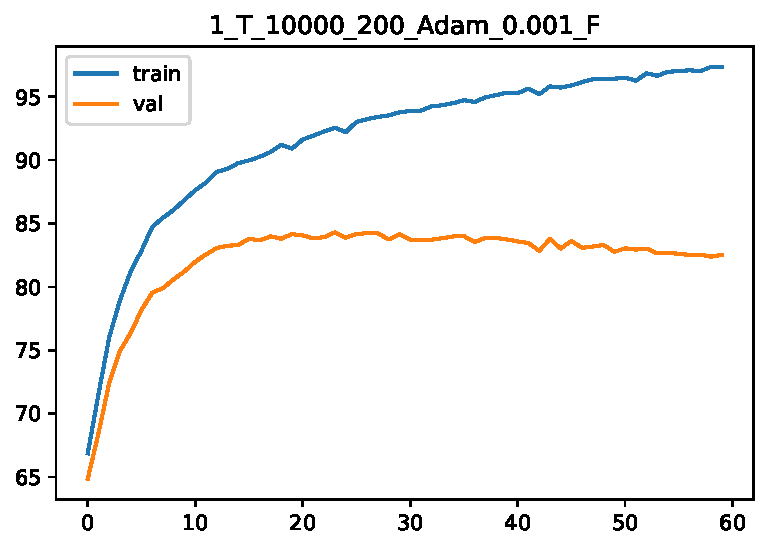
\includegraphics[width = 3cm]{1_T_10000_200_Adam_0001_F.pdf}
}	\\
\subfloat[(20000,200)]{
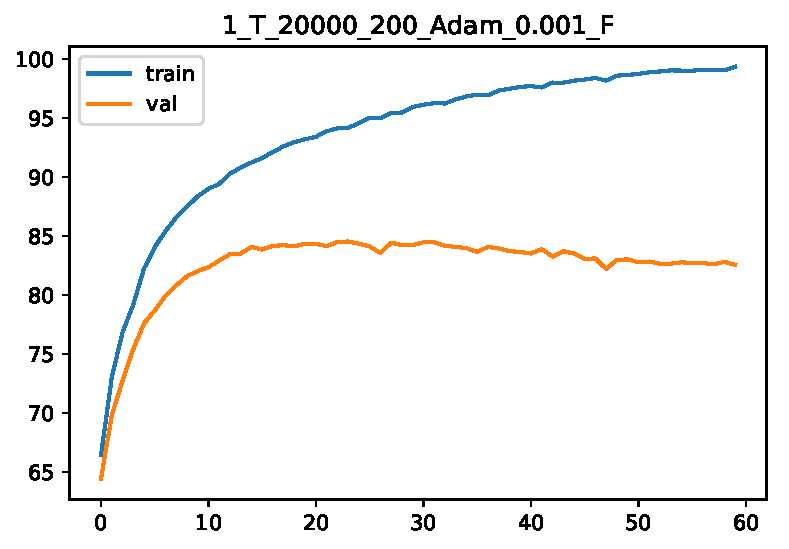
\includegraphics[width = 3cm]{1_T_20000_200_Adam_0001_F.pdf}
}	
\subfloat[(5000,500)]{
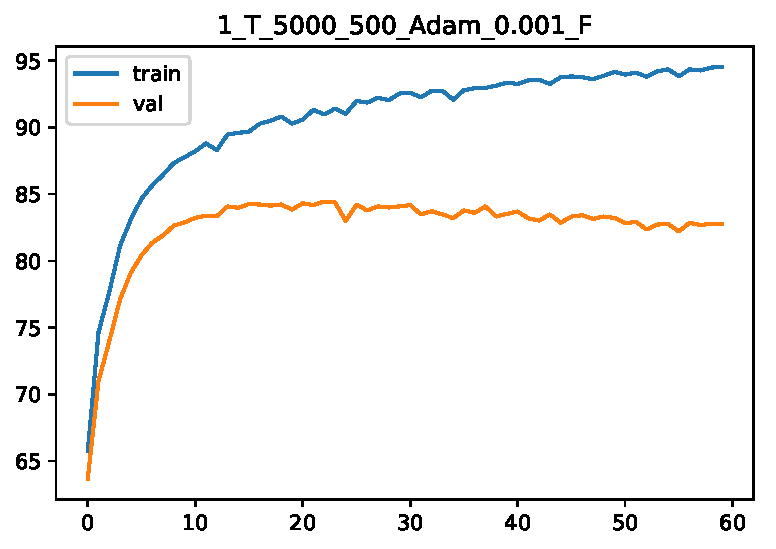
\includegraphics[width = 3cm]{1_T_5000_500_Adam_0001_F.pdf}
}	
\subfloat[(10000,500)]{
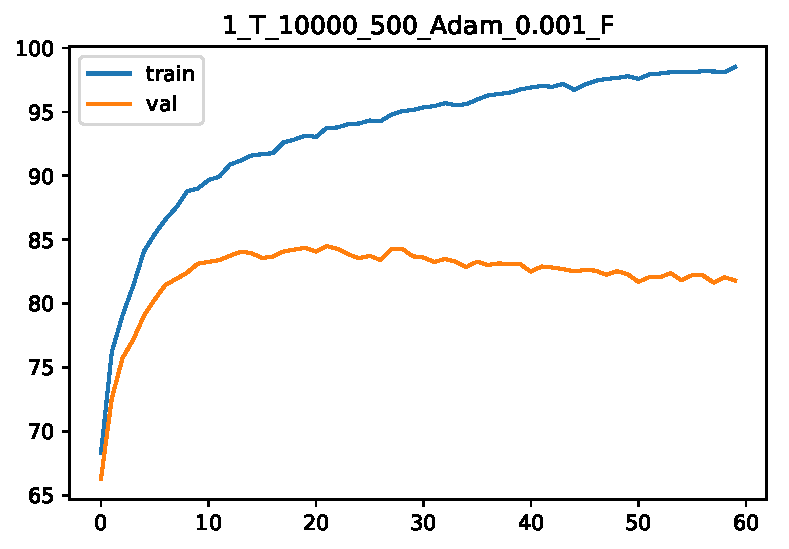
\includegraphics[width = 3cm]{1_T_10000_500_Adam_0001_F.pdf}
}	
\subfloat[(20000,500)]{
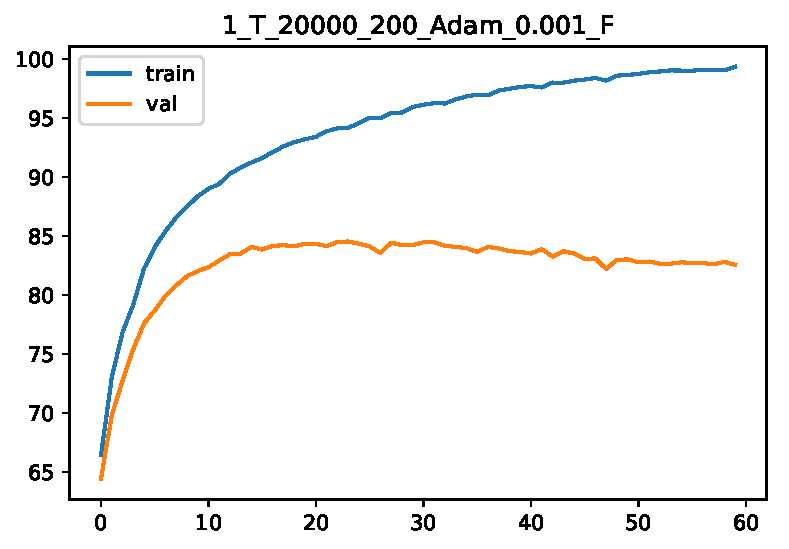
\includegraphics[width = 3cm]{1_T_20000_200_Adam_0001_F.pdf}
}	
\caption{\label{fig:vocab_emd}Vary Vocabulary Size and Embedding Size,  and Fix the Others Learning Curves.}
\end{figure}

We find the best vocab\_size and emd\_size are 5000,200. Generally the vocab\_size and emd\_size do not change the validation accuracy too much. We plot the 9 learning curves in Figure \ref{fig:vocab_emd}.

 
\subsection{Vary Ngram, and Fix the Others}
We use the previously tuned best vocab\_size = 5000 and emd\_size = 200. We keep the optimization hyperparameters unchanged and vary n-grams strategy. The results are shown in Table \ref{tab: ngram}.
\begin{table}[!ht]
\centering
\begin{tabular}{|c|c|c|c|c|c|c|c|}
\hline
n & 1 &\multicolumn{2}{|c|}{2} & \multicolumn{2}{|c|}{3} & \multicolumn{2}{|c|}{4}\\ \hline
all\_gram & doesn't matter & True & False & True & False & True & False \\ \hline
Accuracy & 83.76 & 84.62 & 81.86 & 84.44 & 75.2 & 84.72 & 69.84\\ \hline
\end{tabular}
\caption{\label{tab: ngram}Accuracy on Validation Set When We Vary Ngram, and Fix the Others.}
\end{table}
The best configuration is 4-gram including n-gram with n smaller than 4 with accuracy 84.72 on Validation Set.
\begin{figure}[!ht]
\centering
\subfloat[(1,T)]{
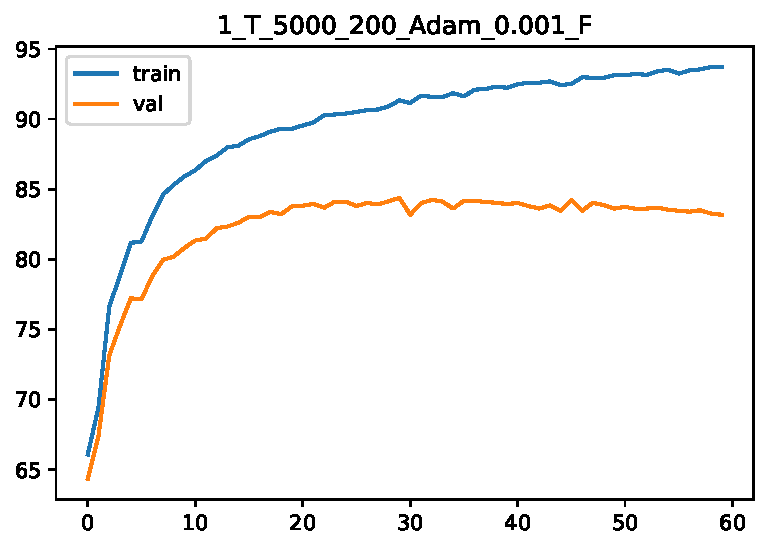
\includegraphics[width = 3cm]{1_T_5000_200_Adam_0001_F.pdf}
}
\subfloat[(2,T)]{
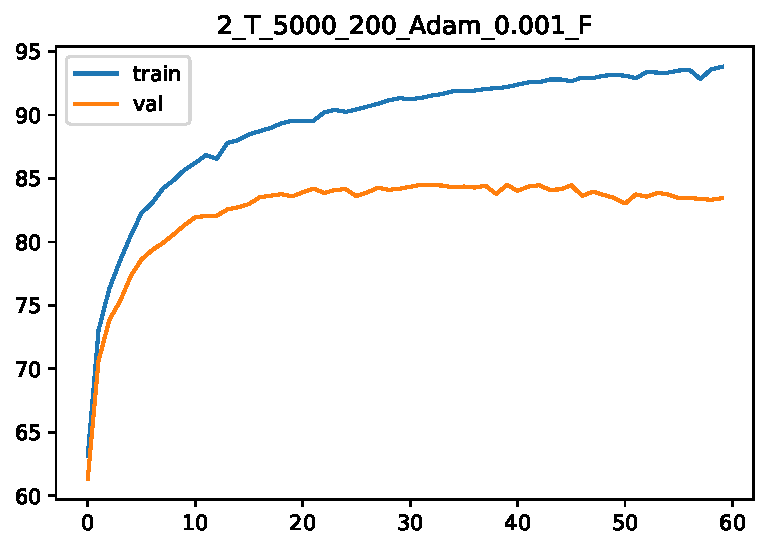
\includegraphics[width = 3cm]{2_T_5000_200_Adam_0001_F.pdf}
}	
\subfloat[(2,F)]{
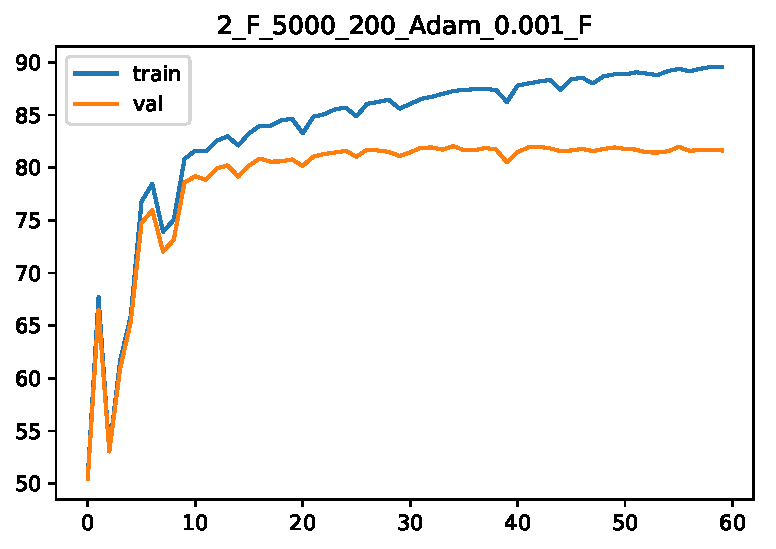
\includegraphics[width = 3cm]{2_F_5000_200_Adam_0001_F.pdf}
}	
\subfloat[(3,T)]{
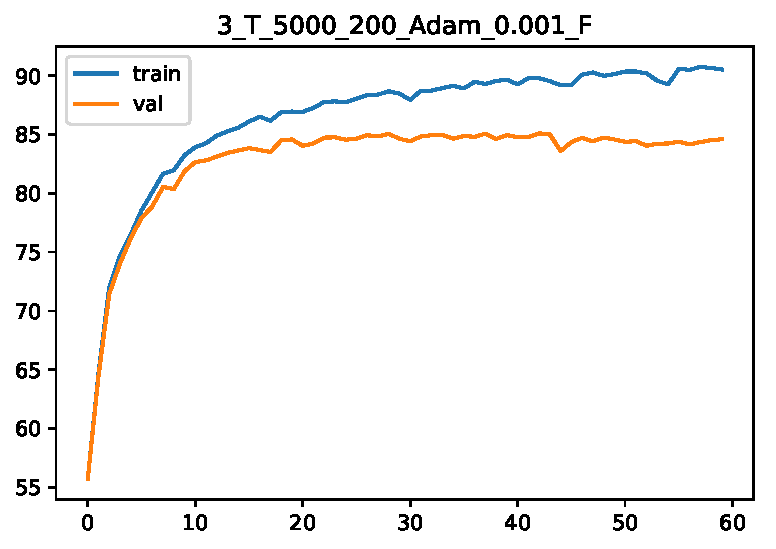
\includegraphics[width = 3cm]{3_T_5000_200_Adam_0001_F.pdf}
}		\\
\subfloat[(3,F)]{
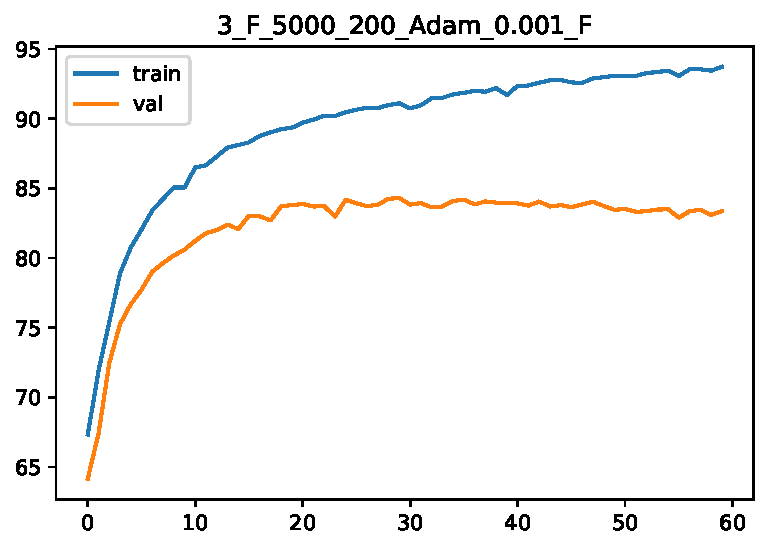
\includegraphics[width = 3cm]{3_F_5000_200_Adam_0001_F.pdf}
}		
\subfloat[(4,T)]{
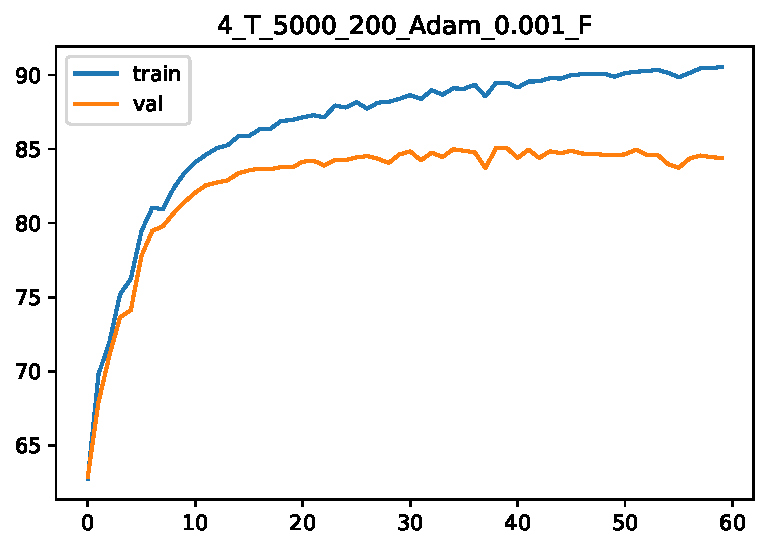
\includegraphics[width = 3cm]{4_T_5000_200_Adam_0001_F.pdf}
}	
\subfloat[(4,F)]{
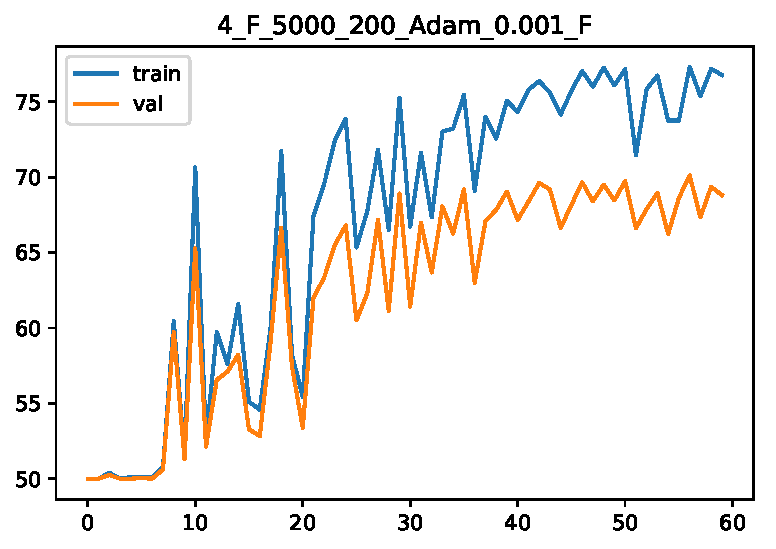
\includegraphics[width = 3cm]{4_F_5000_200_Adam_0001_F.pdf}
}	
\caption{\label{fig:ngram}Vary Ngram, and Fix the Others Learning Curves.}
\end{figure}
We plot the learning curves in Figure \ref{fig:ngram}.
\subsection{Vary Optimization and Fix the Others}
Finally we tune the optimization parameters. We fix n = 2, all\_ngram = False, vocab\_size =5000, emd\_size = 200 and vary optimization parameters.
\begin{table}[!ht]
\centering
\begin{tabular}{|c|c|c|c|c|c|c|c|c|c|c|c|c|}
\hline
Optimizer & \multicolumn{6}{|c|}{SGD} & \multicolumn{6}{|c|}{Adam} \\ \hline
lr\_decay & \multicolumn{3}{|c|}{True}& \multicolumn{3}{|c|}{False} &\multicolumn{3}{|c|}{True}& \multicolumn{3}{|c|}{False}\\ \hline
lr & 0.1 & 0.01 & 0.001 & 0.1 & 0.01 & 0.001 & 0.1 & 0.01 & 0.001 & 0.1 & 0.01 & 0.001\\ \hline
accuracy & 69.42 &64.56 & 59.22&68.18 &64.74 & 59.72&79.4& 81.62& 84.2 &80.3& 81.22 & 84.5 \\ \hline
\end{tabular}
\caption{\label{tab: optim}Accuracy on Validation Set When We Vary Optimization and Fix the Others.}
\end{table}
We show the validation accuracies in Table \ref{tab: optim}. It turns out that our first choice of optimization hyperparameters are the best in the previous two sections. We are lucky! We plot the learning curves in Figure \ref{fig:optim}. Adam prefers smaller learning rate while SGD prefers larger learning rate.
\begin{figure}[!ht]
\centering
\subfloat[(Adam,F,0.001)]{
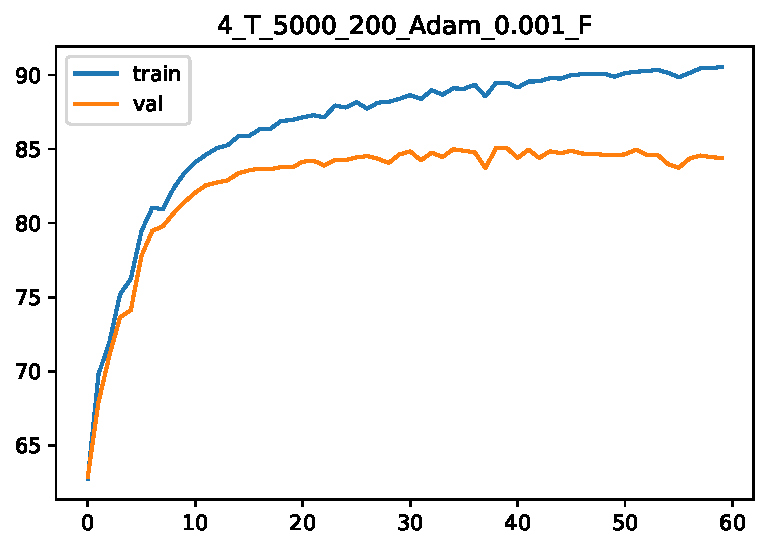
\includegraphics[width = 3cm]{4_T_5000_200_Adam_0001_F.pdf}
}
\subfloat[(Adam,T,0.001)]{
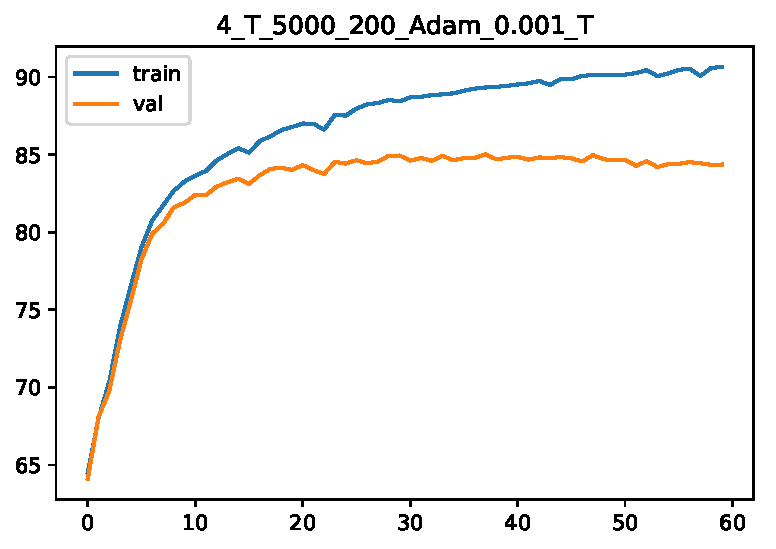
\includegraphics[width = 3cm]{4_T_5000_200_Adam_0001_T.pdf}
}	
\subfloat[(SGD,F,0.001)]{
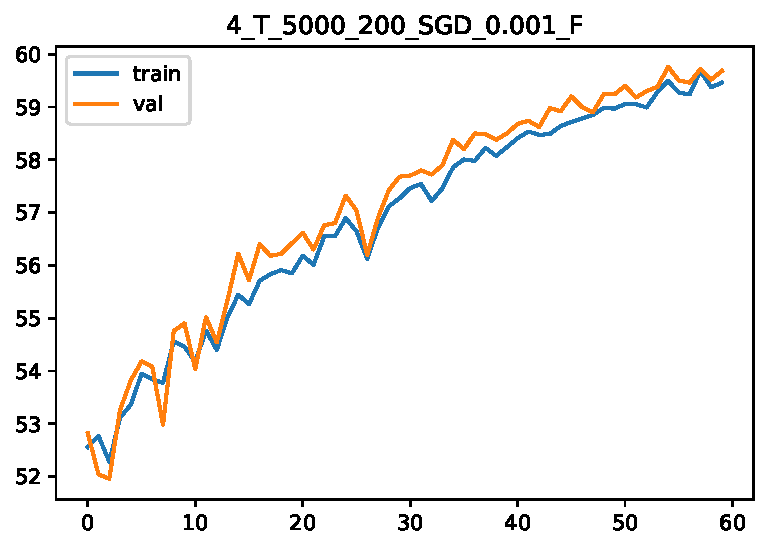
\includegraphics[width = 3cm]{4_T_5000_200_SGD_0001_F.pdf}
}
\subfloat[(SGD,T,0.001)]{
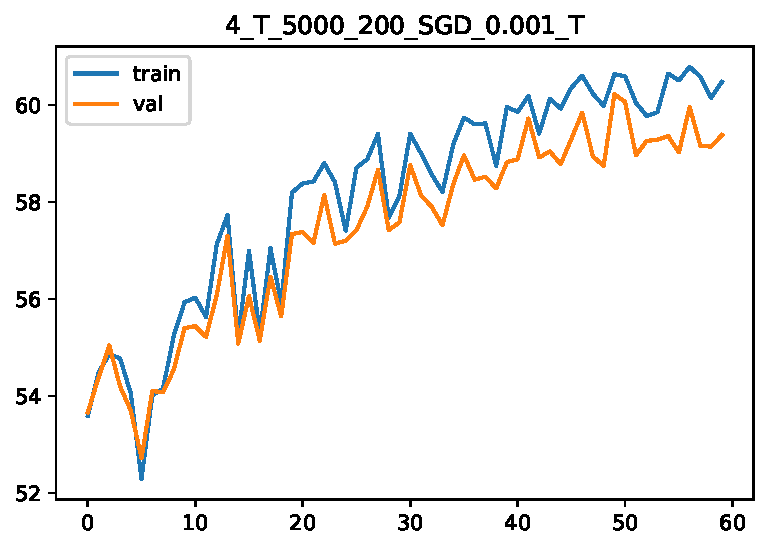
\includegraphics[width = 3cm]{4_T_5000_200_SGD_0001_T.pdf}
}		\\
\subfloat[(Adam,F,0.01)]{
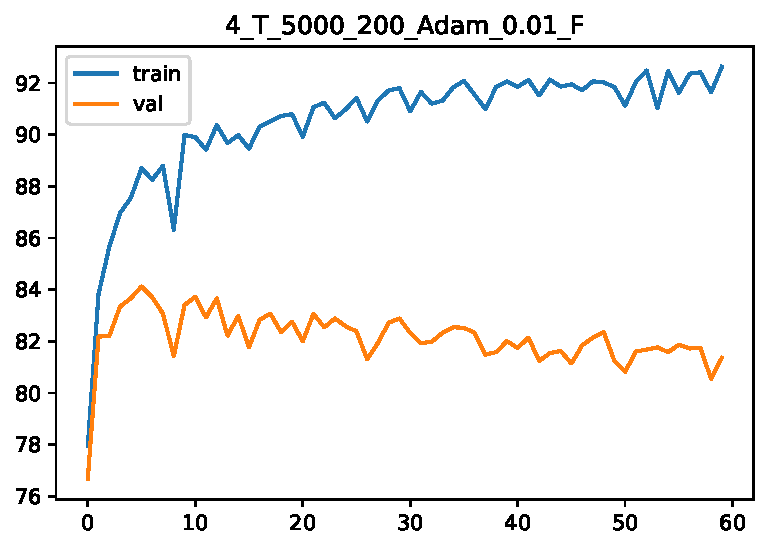
\includegraphics[width = 3cm]{4_T_5000_200_Adam_001_F.pdf}
}
\subfloat[(Adam,T,0.01)]{
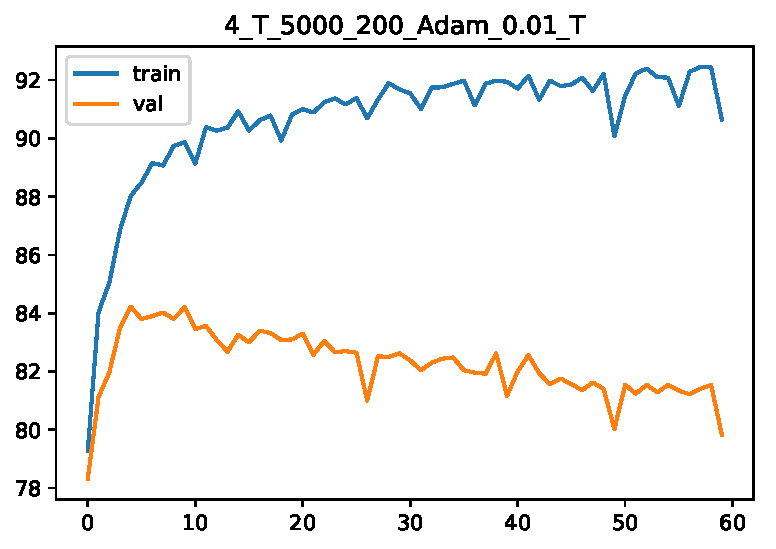
\includegraphics[width = 3cm]{4_T_5000_200_Adam_001_T.pdf}
}	
\subfloat[(SGD,F,0.01)]{
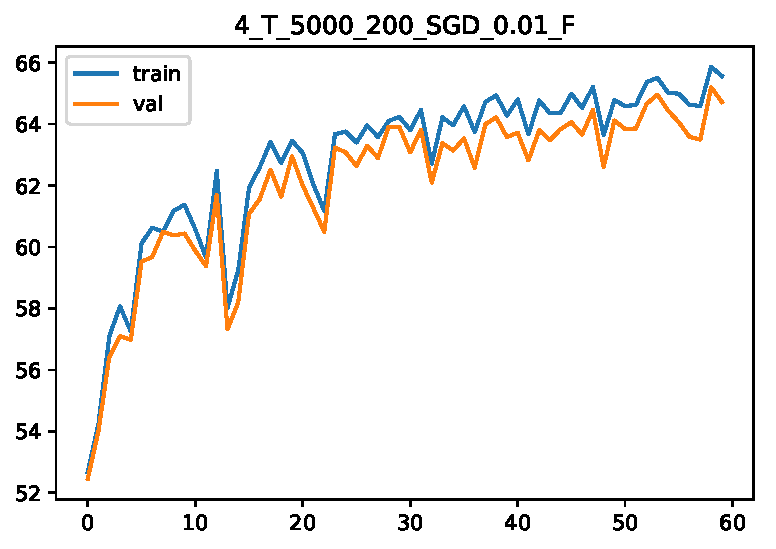
\includegraphics[width = 3cm]{4_T_5000_200_SGD_001_F.pdf}
}
\subfloat[(SGD,T,0.01)]{
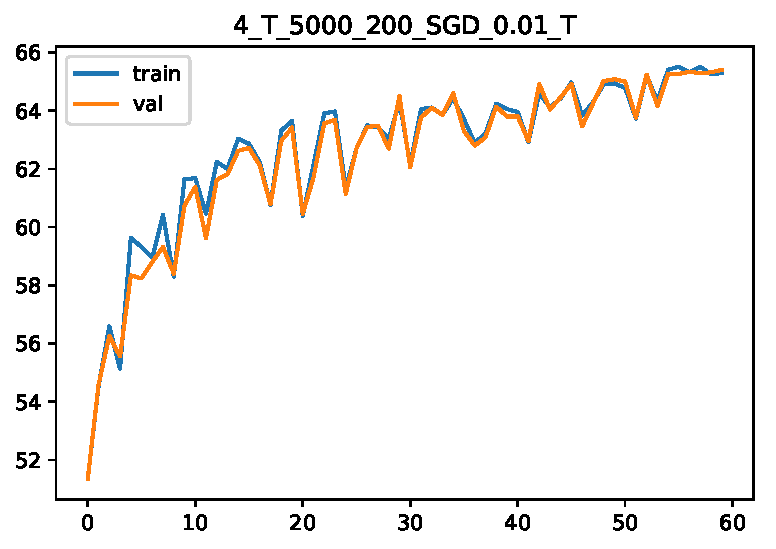
\includegraphics[width = 3cm]{4_T_5000_200_SGD_001_T.pdf}
}		\\
\subfloat[(Adam,F,0.1)]{
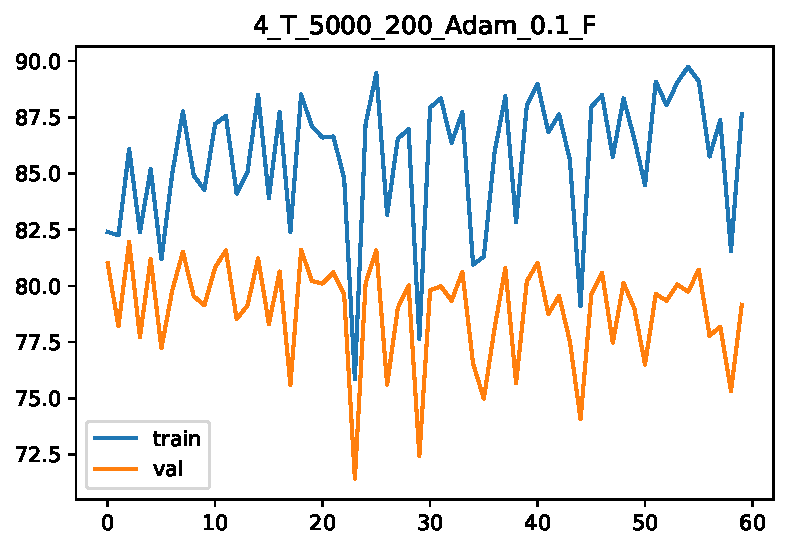
\includegraphics[width = 3cm]{4_T_5000_200_Adam_01_F.pdf}
}
\subfloat[(Adam,T,0.1)]{
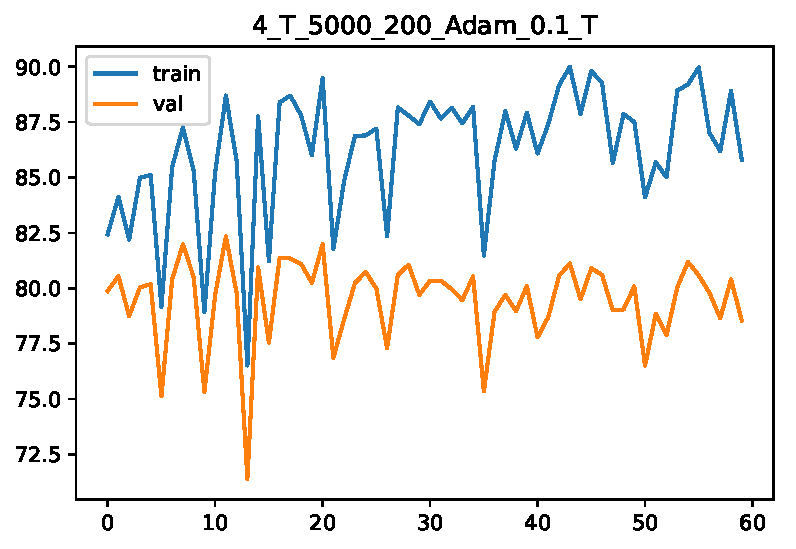
\includegraphics[width = 3cm]{4_T_5000_200_Adam_01_T.pdf}
}	
\subfloat[(SGD,F,0.1)]{
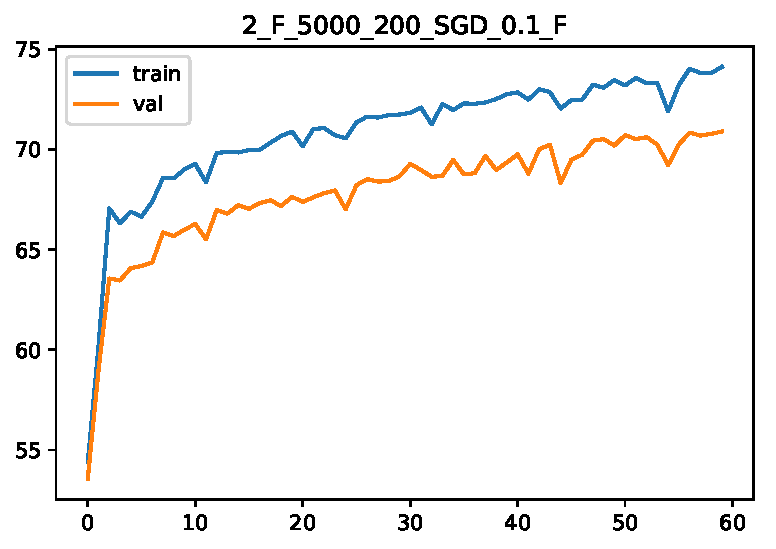
\includegraphics[width = 3cm]{2_F_5000_200_SGD_01_F.pdf}
}
\subfloat[(SGD,T,0.1)]{
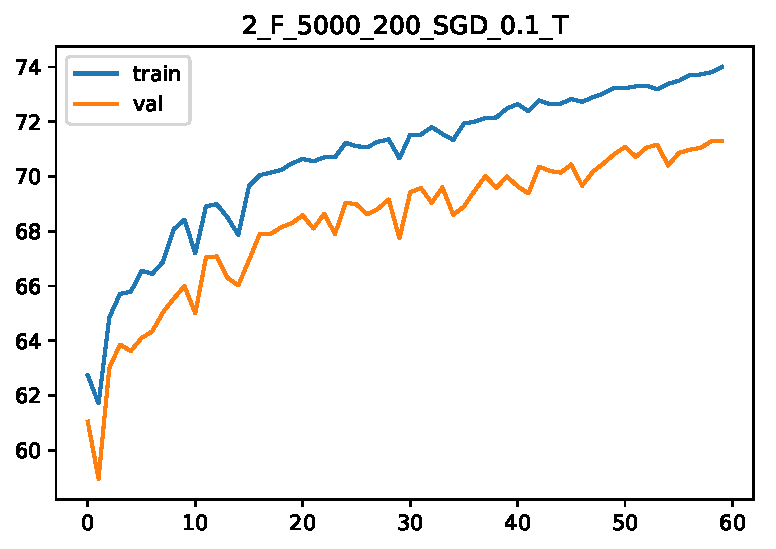
\includegraphics[width = 3cm]{2_F_5000_200_SGD_01_T.pdf}
}
\caption{\label{fig:optim}Vary Optimization and Fix the Others Learning Curves.}
\end{figure}
\subsection{Best Hyperparameters and Test Accuracy}
After ablation hyperparameters search, we have the best hyperparameters combination. They are \{ n=4, all\_ngram = True, max\_vocab\_size = 5000, emd\_size = 200, optimizer = Adam, lr = 0.001, lr\_decay = False\}. The test accuracy we get is 84.604 based on our best hyperparameters.
\subsection{List 3 Correct Predictions and 3 Incorrect Predictions}
Correct Predictions. They are all classified as negative.
\begin{itemize}
\item What is this ? A low budget sex comedy ? Anyway it describes perfectly the people in Spain. They could come up with a better idea, I mean they do this kind of movies since the 60s.. and people like them ! This is neither a teen comedy nor a family one (you can't let your 12 year old watch 2 guys in bed kissing, he'll never want to go to Spain). This should be rated "R", because only people 35+ seem to laugh watching :S I'm truly disappointed, maybe I don't like gays (which is quite an important part of the movie).<br /><br />Foreign humor is awful in films (except Kusturica), stick with doing dramas! If you want a new comedy try Talladega Nights
\item Strange, almost all reviewers are highly positive about this movie. Is it because it's from 1975 and has Chamberlain and Curtis in it and therefore forgive the by times very bad acting and childish ways of storytelling? <br /><br />Maybe it's because some people get sentimental about this film because they have read the book? (I have not read the book, but I don't think that's a problem, film makers never presume that the viewers have read the book). <br /><br />Or is it because I am subconsciously irritated about the fact that English-speaking actors try to behave as their French counterparts?
\item Hey HULU.com is playing the Elvira late night horror show on their site and this movie is their under the Name Monsteroid, good fun to watch Elvira comment on this Crappy movie ....Have Fun with bad movies. Anyways this movie really has very little value other than to see how bad the 70's were for horror flicks Bad Effects, Bad Dialog, just bad movie making. Avoid this unless you want to laugh at it. While you are at HULU check out the other movies that are their right now there is 10 episodes and some are pretty decent movies with good plots and production and you can watch a lot of them in 480p as long as you have a decent speed connection.
\end{itemize}
Incorrect Predictions. They should be negative but my model predicts them to be positive.
\begin{itemize}
\item I can not believe such slanted, jingoistic material is getting passed off to Americans as art house material. Early on, from such telling lines like "we want to make sure they are playing for the right team" and manipulative framing and lighting, A Love Divided shows it's true face. The crass manner in which the Irish Catholics are shown as hegemonic, the Protestants as peaceful and downtrodden, is as poor a representation of history as early US westerns that depict the struggle between cowboys and American Indians. The truth of the story is distorted with the stereotypes and outright vilification of the Irish Catholics in the story; a corruption admitted by the filmmakers themselves! It is sad that people today still think that they can win moral sway by making a film so easily recognized for it's obvious intent, so far from attempting art. This film has no business being anywhere in any legitimate cinema or library.
\item I've seen the original non-dubbed German version and I was surprised how bad this movie actually is. Thinking I had seen my share of bad movies like Ghoulies 2, Rabid Grannies, Zombie Lake and such, nothing could've prepared me for this! It really was a pain to sit through this flick, as there's no plot, no good acting and even the special effects aren't convincing, especially the so-called zombies, wearing nothing more than white make-up and their old clothes, so their good set wouldn't be ruined by ketchup and marmalade stains. <br /><br />If you really want to waste 90 minutes of your life, then watch it, for all the others, don't do it, because you WILL regret it!
\item Outside of the fact that George Lopez is a pretentious jerk, his show is terrible.<br /><br />Nothing about Lopez has ever been funny. I have watched his stand-up and have never uttered any resemblance to a laugh.<br /><br />His stuff comes across as vindictive and his animosity towards white people oozes out of every single pore of his body.<br /><br />I have laughed at white people jokes from many a comedian and love many of them.<br /><br />This guy has a grudge that won't end.<br /><br />I feel bad for Hispanics who have only this show to represent themselves.<br /><br />The shows plots are always cookie cutter with an Hispanic accent.<br /><br />Canned laugh at the dumbest comments and scenes.<br /><br />Might be why this show is always on at 2AM in replay.	
\end{itemize}

\section{Extra Points}
\subsection{Extra Hyperparamter Search}
We notice there is an extra hyperparameter in the code. That is MAX\_SENTENCE\_LENGTH. We choose three different values 150,200, and 250. We keep the other hyperparameters to be the optimal one we get in the previous section. Pleas see the code in $\texttt{hw1.ipynb}$ for reference. When we increase the MAX\_SENTENCE\_LENGTH from 150 ,200 to 250. The validation accuracy rises from 82.78, 84.06 tp 85.58. So the MAX\_SENTENCE\_LENGTH is an important hyperparameter. And the test accuracy for MAX\_SENTENCE\_LENGTH=250 model is 85.748.

There is another hyperparameter number of the epochs.  We try number of epochs 5 instead of 10 . We get 85.28 on validation set and 85.916 on test set. This does not improve the previous accuracy. So the final \textbf{test score} in this homework is \textbf{85.748}. 
\subsection{Train 1-10 rating}
Instead of training negative and positive reviews, we could also train a 1-10 rating. In order to do so, we train a 10 class classifier. Pleas see the code in $\texttt{hw1.ipynb}$ for reference. I use the previous configuration from binary classification. It turns out that the accuracy is very low. I think the reason is that the model is two simple for 10-class classification. The validation accuracy is the 32.32. and the test accuracy is 34.4056








